\documentclass[]{article}
\usepackage{lmodern}
\usepackage{amssymb,amsmath}
\usepackage{ifxetex,ifluatex}
\usepackage{fixltx2e} % provides \textsubscript
\ifnum 0\ifxetex 1\fi\ifluatex 1\fi=0 % if pdftex
  \usepackage[T1]{fontenc}
  \usepackage[utf8]{inputenc}
\else % if luatex or xelatex
  \ifxetex
    \usepackage{mathspec}
  \else
    \usepackage{fontspec}
  \fi
  \defaultfontfeatures{Ligatures=TeX,Scale=MatchLowercase}
\fi
% use upquote if available, for straight quotes in verbatim environments
\IfFileExists{upquote.sty}{\usepackage{upquote}}{}
% use microtype if available
\IfFileExists{microtype.sty}{%
\usepackage{microtype}
\UseMicrotypeSet[protrusion]{basicmath} % disable protrusion for tt fonts
}{}
\usepackage[margin=1in]{geometry}
\usepackage{hyperref}
\hypersetup{unicode=true,
            pdftitle={MATH 4753 Project 2},
            pdfauthor={Justin Kleiber},
            pdfborder={0 0 0},
            breaklinks=true}
\urlstyle{same}  % don't use monospace font for urls
\usepackage{color}
\usepackage{fancyvrb}
\newcommand{\VerbBar}{|}
\newcommand{\VERB}{\Verb[commandchars=\\\{\}]}
\DefineVerbatimEnvironment{Highlighting}{Verbatim}{commandchars=\\\{\}}
% Add ',fontsize=\small' for more characters per line
\usepackage{framed}
\definecolor{shadecolor}{RGB}{248,248,248}
\newenvironment{Shaded}{\begin{snugshade}}{\end{snugshade}}
\newcommand{\AlertTok}[1]{\textcolor[rgb]{0.94,0.16,0.16}{#1}}
\newcommand{\AnnotationTok}[1]{\textcolor[rgb]{0.56,0.35,0.01}{\textbf{\textit{#1}}}}
\newcommand{\AttributeTok}[1]{\textcolor[rgb]{0.77,0.63,0.00}{#1}}
\newcommand{\BaseNTok}[1]{\textcolor[rgb]{0.00,0.00,0.81}{#1}}
\newcommand{\BuiltInTok}[1]{#1}
\newcommand{\CharTok}[1]{\textcolor[rgb]{0.31,0.60,0.02}{#1}}
\newcommand{\CommentTok}[1]{\textcolor[rgb]{0.56,0.35,0.01}{\textit{#1}}}
\newcommand{\CommentVarTok}[1]{\textcolor[rgb]{0.56,0.35,0.01}{\textbf{\textit{#1}}}}
\newcommand{\ConstantTok}[1]{\textcolor[rgb]{0.00,0.00,0.00}{#1}}
\newcommand{\ControlFlowTok}[1]{\textcolor[rgb]{0.13,0.29,0.53}{\textbf{#1}}}
\newcommand{\DataTypeTok}[1]{\textcolor[rgb]{0.13,0.29,0.53}{#1}}
\newcommand{\DecValTok}[1]{\textcolor[rgb]{0.00,0.00,0.81}{#1}}
\newcommand{\DocumentationTok}[1]{\textcolor[rgb]{0.56,0.35,0.01}{\textbf{\textit{#1}}}}
\newcommand{\ErrorTok}[1]{\textcolor[rgb]{0.64,0.00,0.00}{\textbf{#1}}}
\newcommand{\ExtensionTok}[1]{#1}
\newcommand{\FloatTok}[1]{\textcolor[rgb]{0.00,0.00,0.81}{#1}}
\newcommand{\FunctionTok}[1]{\textcolor[rgb]{0.00,0.00,0.00}{#1}}
\newcommand{\ImportTok}[1]{#1}
\newcommand{\InformationTok}[1]{\textcolor[rgb]{0.56,0.35,0.01}{\textbf{\textit{#1}}}}
\newcommand{\KeywordTok}[1]{\textcolor[rgb]{0.13,0.29,0.53}{\textbf{#1}}}
\newcommand{\NormalTok}[1]{#1}
\newcommand{\OperatorTok}[1]{\textcolor[rgb]{0.81,0.36,0.00}{\textbf{#1}}}
\newcommand{\OtherTok}[1]{\textcolor[rgb]{0.56,0.35,0.01}{#1}}
\newcommand{\PreprocessorTok}[1]{\textcolor[rgb]{0.56,0.35,0.01}{\textit{#1}}}
\newcommand{\RegionMarkerTok}[1]{#1}
\newcommand{\SpecialCharTok}[1]{\textcolor[rgb]{0.00,0.00,0.00}{#1}}
\newcommand{\SpecialStringTok}[1]{\textcolor[rgb]{0.31,0.60,0.02}{#1}}
\newcommand{\StringTok}[1]{\textcolor[rgb]{0.31,0.60,0.02}{#1}}
\newcommand{\VariableTok}[1]{\textcolor[rgb]{0.00,0.00,0.00}{#1}}
\newcommand{\VerbatimStringTok}[1]{\textcolor[rgb]{0.31,0.60,0.02}{#1}}
\newcommand{\WarningTok}[1]{\textcolor[rgb]{0.56,0.35,0.01}{\textbf{\textit{#1}}}}
\usepackage{graphicx,grffile}
\makeatletter
\def\maxwidth{\ifdim\Gin@nat@width>\linewidth\linewidth\else\Gin@nat@width\fi}
\def\maxheight{\ifdim\Gin@nat@height>\textheight\textheight\else\Gin@nat@height\fi}
\makeatother
% Scale images if necessary, so that they will not overflow the page
% margins by default, and it is still possible to overwrite the defaults
% using explicit options in \includegraphics[width, height, ...]{}
\setkeys{Gin}{width=\maxwidth,height=\maxheight,keepaspectratio}
\IfFileExists{parskip.sty}{%
\usepackage{parskip}
}{% else
\setlength{\parindent}{0pt}
\setlength{\parskip}{6pt plus 2pt minus 1pt}
}
\setlength{\emergencystretch}{3em}  % prevent overfull lines
\providecommand{\tightlist}{%
  \setlength{\itemsep}{0pt}\setlength{\parskip}{0pt}}
\setcounter{secnumdepth}{0}
% Redefines (sub)paragraphs to behave more like sections
\ifx\paragraph\undefined\else
\let\oldparagraph\paragraph
\renewcommand{\paragraph}[1]{\oldparagraph{#1}\mbox{}}
\fi
\ifx\subparagraph\undefined\else
\let\oldsubparagraph\subparagraph
\renewcommand{\subparagraph}[1]{\oldsubparagraph{#1}\mbox{}}
\fi

%%% Use protect on footnotes to avoid problems with footnotes in titles
\let\rmarkdownfootnote\footnote%
\def\footnote{\protect\rmarkdownfootnote}

%%% Change title format to be more compact
\usepackage{titling}

% Create subtitle command for use in maketitle
\providecommand{\subtitle}[1]{
  \posttitle{
    \begin{center}\large#1\end{center}
    }
}

\setlength{\droptitle}{-2em}

  \title{MATH 4753 Project 2}
    \pretitle{\vspace{\droptitle}\centering\huge}
  \posttitle{\par}
    \author{Justin Kleiber}
    \preauthor{\centering\large\emph}
  \postauthor{\par}
      \predate{\centering\large\emph}
  \postdate{\par}
    \date{10 November, 2019}


\begin{document}
\maketitle
\begin{abstract}
This project is all about applications of SLR to real data using R
\end{abstract}

{
\setcounter{tocdepth}{4}
\tableofcontents
}
\begin{figure}
\centering
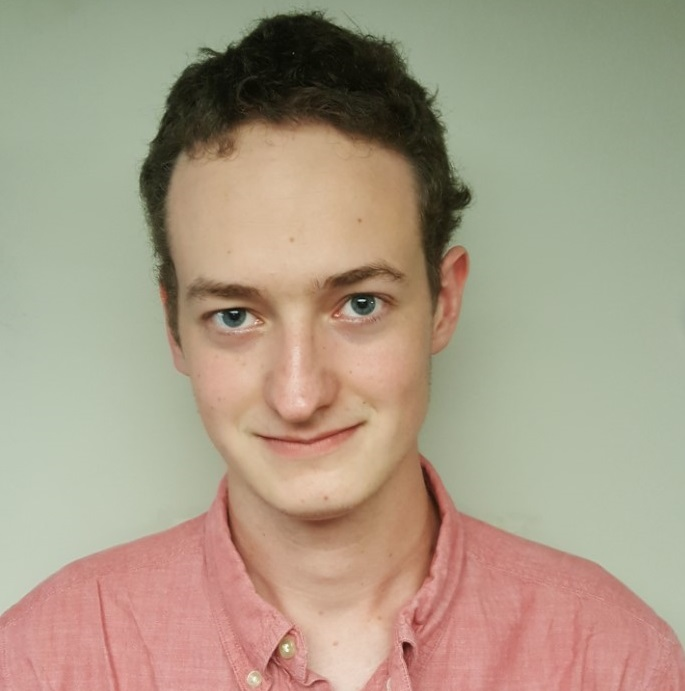
\includegraphics[width=0.2\textwidth,height=\textheight]{justin.jpg}
\caption{Justin Kleiber}
\end{figure}

\hypertarget{my-video}{%
\section{My Video}\label{my-video}}

\hypertarget{introduction}{%
\section{Introduction}\label{introduction}}

When applying for jobs, applicants are often asked about their desired
salary, or their salary history. This is a tactic called ``anchoring'',
where a potential employer tries to pin the future salary negotiations
with the applicant to a low value in order to pay the lowest possible
price for future labor (Kahneman (1992)). Research studies have shown
that such an approach influences negotiations, even if the anchor point
is extreme (Thorsteinson (2011)).

Asking about salary history in particular has negative outcomes for
women, leading some cities, states and companies to outlaw the question
entirely during the interview stages. Furthermore, it has been shown
that women, who generally participate less in salary negotiations than
their male counterparts, become more likely to negotiate their salary
when armed with information about what they deserve to earn (Douglas and
Miller (2015)).

By applying simple linear regression to a given salary data set, it is
predicted that such a model can accurately predict salary based on the
amount of work experience an employee has. This model then can be used
by the employee to achieve a more favorable outcome during salary
negotiations, as a reasonable salary estimate can be predicted.

\hypertarget{variables}{%
\subsection{Variables}\label{variables}}

The two variables of interest are years of experience, and the salary
earned.

\begin{Shaded}
\begin{Highlighting}[]
\NormalTok{salary =}\StringTok{ }\KeywordTok{read.csv}\NormalTok{(}\StringTok{"Salary_Data.csv"}\NormalTok{)}

\KeywordTok{library}\NormalTok{(DT)}
\KeywordTok{datatable}\NormalTok{(}
\NormalTok{  salary,}\DataTypeTok{filter =} \StringTok{'top'}\NormalTok{, }\DataTypeTok{options =} \KeywordTok{list}\NormalTok{(}
  \DataTypeTok{pageLength =} \DecValTok{5}\NormalTok{, }\DataTypeTok{autoWidth =} \OtherTok{TRUE}\NormalTok{, }\DataTypeTok{editable =} \OtherTok{TRUE}\NormalTok{, }\DataTypeTok{dom =} \StringTok{'Bfrtip'}\NormalTok{,}
    \DataTypeTok{buttons =} \KeywordTok{c}\NormalTok{(}\StringTok{'copy'}\NormalTok{, }\StringTok{'csv'}\NormalTok{, }\StringTok{'excel'}\NormalTok{, }\StringTok{'pdf'}\NormalTok{, }\StringTok{'print'}\NormalTok{)),}
\DataTypeTok{caption =}\NormalTok{ htmltools}\OperatorTok{::}\NormalTok{tags}\OperatorTok{$}\KeywordTok{caption}\NormalTok{(}
    \DataTypeTok{style =} \StringTok{'caption-side: bottom; text-align: center;'}\NormalTok{,}
    \StringTok{'Table 2: '}\NormalTok{, htmltools}\OperatorTok{::}\KeywordTok{em}\NormalTok{(}\StringTok{'This is a simple caption for the table.'}\NormalTok{)}
\NormalTok{  )}
\NormalTok{) }\OperatorTok
\StringTok{  }\KeywordTok{formatStyle}\NormalTok{(}\StringTok{'Salary'}\NormalTok{,  }\DataTypeTok{color =} \StringTok{'red'}\NormalTok{, }\DataTypeTok{backgroundColor =} \StringTok{'orange'}\NormalTok{, }\DataTypeTok{fontWeight =} \StringTok{'bold'}\NormalTok{)}
\end{Highlighting}
\end{Shaded}

\begin{verbatim}
## PhantomJS not found. You can install it with webshot::install_phantomjs(). If it is installed, please make sure the phantomjs executable can be found via the PATH variable.
\end{verbatim}

\hypertarget{htmlwidget-d735d2c36a342a935ea7}{}

\hypertarget{plot}{%
\subsubsection{Plot}\label{plot}}

\begin{Shaded}
\begin{Highlighting}[]
\KeywordTok{library}\NormalTok{(ggplot2)}
\NormalTok{g =}\StringTok{ }\KeywordTok{ggplot}\NormalTok{(salary, }\KeywordTok{aes}\NormalTok{(}\DataTypeTok{x =}\NormalTok{ YearsExperience, }\DataTypeTok{y =}\NormalTok{ Salary)) }\OperatorTok{+}\StringTok{ }\KeywordTok{geom_point}\NormalTok{()}
\NormalTok{g =}\StringTok{ }\NormalTok{g }\OperatorTok{+}\StringTok{ }\KeywordTok{geom_smooth}\NormalTok{(}\DataTypeTok{method =} \StringTok{"loess"}\NormalTok{)}
\NormalTok{g}
\end{Highlighting}
\end{Shaded}

\begin{figure}

{\centering \includegraphics{Project2_files/figure-latex/carcharacteristics-1} 

}

\caption{Graph of data with loess smoother}\label{fig:carcharacteristics}
\end{figure}

\hypertarget{data-collection}{%
\subsection{Data Collection}\label{data-collection}}

The salary data was sourced from Kaggle, a data science website with
many interesting data sets.

\hypertarget{reason-for-collection}{%
\subsection{Reason For Collection}\label{reason-for-collection}}

This data was originally collected to compare the salaries of many
professionals, each at different career stages.

\hypertarget{interest}{%
\subsection{Interest}\label{interest}}

This data provides an opportunity to study the efficacy of simple linear
regression in predicting a worker's salary before the worker goes into
salary negotiations.

\hypertarget{problem}{%
\subsection{Problem}\label{problem}}

Employers frequently attempt to exploit employees by anchoring salary
negotiations to an employee's past rather than considering the
employee's current career stage.

\hypertarget{hypothesis}{%
\subsection{Hypothesis}\label{hypothesis}}

Simple linear regression can be used to provide job applicants and
current employees with accurate salary information, with which they can
use to better negotiate their own salary.

\hypertarget{theory-needed-to-carry-out-slr}{%
\section{Theory needed to carry out
SLR}\label{theory-needed-to-carry-out-slr}}

A linear combination is a weighted composition of potentially many
variables, as shown below.

\[
y = \beta_0 + \beta_1x_1 + ...+\beta_nx^n = \sum_{i=0}^n{\beta_ix^i}
\]

From (``Simple Linear Regression'' 2008), and the equation for a linear
combination, it is determined that the output, \(y_i\), of a linear
model given a single input variable, \(x_i\), is as follows:

\[
y_i = \beta_0 + \beta_1x_i + \epsilon_i
\]

Where \(\epsilon_i\) represents the error of the model. This equation is
known as the regression line. This equation can be used to find the
expected value of \(y_i\) given the input variable \(x_i\). More
formally:

\[
\begin{eqnarray}
E(y_i | x_i) &=& E(\beta_0 + \beta_1x_i + \epsilon_i)\\
E(y_i | x_i) &=& E(\beta_0) + E(\beta_1x_i) + E(\epsilon_i)\\
E(y_i | x_i) &=& \beta_0 + \beta_1x_i\\
\end{eqnarray}
\]

which aligns with the equation for a linear combination. However, this
derivation relies on the assumption that
\(\epsilon_i ~ N(0, \sigma^2)\). In other words, the error of the model
must be normally distributed with a mean of zero in order to be perfect.
As most models are not perfect, they must be validated to see how well
they fit the given data.

\hypertarget{validity-of-model}{%
\section{Validity of Model}\label{validity-of-model}}

A linear model of the salary data is constructed using the following R
code

\begin{Shaded}
\begin{Highlighting}[]
\NormalTok{salary.lm =}\StringTok{ }\KeywordTok{lm}\NormalTok{(Salary}\OperatorTok{~}\NormalTok{YearsExperience, }\DataTypeTok{data =}\NormalTok{ salary)}
\end{Highlighting}
\end{Shaded}

This model will undergo a variety of methods to confirm its validity in
delivering a prediction about salary data.

\hypertarget{straight-trendline-verification}{%
\subsection{Straight trendline
verification}\label{straight-trendline-verification}}

One assumption of simple linear regression with one input variable is
that the model should be a straight line. This assumption is verified
using \texttt{trendscatter}

\begin{Shaded}
\begin{Highlighting}[]
\CommentTok{# Load the s20x library and make three trendline scatter plots}
\KeywordTok{library}\NormalTok{(s20x)}
\KeywordTok{layout}\NormalTok{(}\KeywordTok{matrix}\NormalTok{(}\DecValTok{1}\OperatorTok{:}\DecValTok{3}\NormalTok{, }\DataTypeTok{nrow =} \DecValTok{3}\NormalTok{, }\DataTypeTok{ncol =} \DecValTok{1}\NormalTok{))}
\KeywordTok{trendscatter}\NormalTok{(Salary}\OperatorTok{~}\NormalTok{YearsExperience, }\DataTypeTok{f =} \FloatTok{0.5}\NormalTok{, }\DataTypeTok{data =}\NormalTok{ salary)}
\KeywordTok{trendscatter}\NormalTok{(Salary}\OperatorTok{~}\NormalTok{YearsExperience, }\DataTypeTok{f =} \FloatTok{0.7}\NormalTok{, }\DataTypeTok{data =}\NormalTok{ salary)}
\KeywordTok{trendscatter}\NormalTok{(Salary}\OperatorTok{~}\NormalTok{YearsExperience, }\DataTypeTok{f =} \FloatTok{0.9}\NormalTok{, }\DataTypeTok{data =}\NormalTok{ salary)}
\end{Highlighting}
\end{Shaded}

\includegraphics{Project2_files/figure-latex/unnamed-chunk-2-1.pdf}

From the \texttt{trendscatter} function calls above and the plots they
output, the assumption that the trendline is straight is reasonable.

\hypertarget{normally-distributed-errors}{%
\subsection{Normally Distributed
Errors}\label{normally-distributed-errors}}

For the model to work, the errors in the model need to be distributed
normal, as shown below.

\[\epsilon_i \sim N(0,\sigma^2)\]

This section will seek to prove the normal distribution of the error
using the Shapiro-Wilk test.

\hypertarget{shapiro-wilk-test}{%
\subsubsection{Shapiro-Wilk Test}\label{shapiro-wilk-test}}

To perform the shapiro-wilk test on the errors, the \texttt{normcheck}
function in R is employed:

\begin{Shaded}
\begin{Highlighting}[]
\CommentTok{# Test the normality of the linear model}
\KeywordTok{normcheck}\NormalTok{(salary.lm, }\DataTypeTok{shapiro.wilk =} \OtherTok{TRUE}\NormalTok{)}
\end{Highlighting}
\end{Shaded}

\includegraphics{Project2_files/figure-latex/unnamed-chunk-3-1.pdf}

As the null-hypothesis of this particular Shapiro-Wilk test is that the
error is normally distributed, and the p-value returned by the
\texttt{normcheck} function is much greater than 0.05, it is reasonable
to accept the null hypothesis as plausible. Therefore, the error being
normally distributed is plausible.

\hypertarget{constant-variance-verification}{%
\subsection{Constant Variance
Verification}\label{constant-variance-verification}}

To show the constant variance of the error, the residuals must be
plotted against the fitted values generated by the model. First the
residuals and the fitted values are found using R:

\begin{Shaded}
\begin{Highlighting}[]
\CommentTok{# Residuals}
\NormalTok{salary.res =}\StringTok{ }\KeywordTok{residuals}\NormalTok{(salary.lm)}

\CommentTok{# Fitted values}
\NormalTok{salary.fit =}\StringTok{ }\KeywordTok{fitted}\NormalTok{(salary.lm)}
\end{Highlighting}
\end{Shaded}

Then, the fitted values of the model and the residuals are plotted
against each other

\begin{Shaded}
\begin{Highlighting}[]
\CommentTok{# Plot residuals vs fitted values}
\KeywordTok{plot}\NormalTok{(salary.fit, salary.res)}
\end{Highlighting}
\end{Shaded}

\includegraphics{Project2_files/figure-latex/unnamed-chunk-5-1.pdf}

\begin{Shaded}
\begin{Highlighting}[]
\KeywordTok{trendscatter}\NormalTok{(salary.fit, salary.res, }\DataTypeTok{f =} \DecValTok{1}\NormalTok{)}
\end{Highlighting}
\end{Shaded}

\includegraphics{Project2_files/figure-latex/unnamed-chunk-5-2.pdf}

This shows that the variance of the error is near constant, which will
make the model much more accurate.

\hypertarget{zero-mean-value-of-epsilon}{%
\subsection{\texorpdfstring{Zero mean value of
\(\epsilon\)}{Zero mean value of \textbackslash epsilon}}\label{zero-mean-value-of-epsilon}}

The mean value of the errors must be zero for the model to be valid. The
mean of the errors can be found by first finding the residuals, and then
finding the mean of the residuals.

\begin{Shaded}
\begin{Highlighting}[]
\NormalTok{salary.res =}\StringTok{ }\KeywordTok{residuals}\NormalTok{(salary.lm)}
\KeywordTok{mean}\NormalTok{(salary.res)}
\end{Highlighting}
\end{Shaded}

\begin{verbatim}
## [1] -2.615537e-13
\end{verbatim}

As shown, the mean of the residuals is very close to 0. In fact, if
floating point precision error in computers is considered, this value is
zero.

\hypertarget{data-independence}{%
\subsection{Data Independence}\label{data-independence}}

\hypertarget{model-selection-if-you-compared-models}{%
\section{Model selection if you compared
models}\label{model-selection-if-you-compared-models}}

\hypertarget{use-adjusted-r2}{%
\subsection{\texorpdfstring{Use adjusted
\(R^2\)}{Use adjusted R\^{}2}}\label{use-adjusted-r2}}

\[R_{adj}^2 =\]

\hypertarget{analysis-of-the-data}{%
\section{Analysis of the data}\label{analysis-of-the-data}}

\hypertarget{make-sure-you-include-many-great-plots}{%
\subsection{Make sure you include many great
plots}\label{make-sure-you-include-many-great-plots}}

\hypertarget{add-the-trend-to-the-data}{%
\subsection{Add the trend to the data}\label{add-the-trend-to-the-data}}

\hypertarget{summary-lm-object}{%
\subsection{Summary lm object}\label{summary-lm-object}}

\begin{Shaded}
\begin{Highlighting}[]
\KeywordTok{summary}\NormalTok{(salary.lm)}
\end{Highlighting}
\end{Shaded}

\begin{verbatim}
## 
## Call:
## lm(formula = Salary ~ YearsExperience, data = salary)
## 
## Residuals:
##     Min      1Q  Median      3Q     Max 
## -7958.0 -4088.5  -459.9  3372.6 11448.0 
## 
## Coefficients:
##                 Estimate Std. Error t value Pr(>|t|)    
## (Intercept)      25792.2     2273.1   11.35 5.51e-12 ***
## YearsExperience   9450.0      378.8   24.95  < 2e-16 ***
## ---
## Signif. codes:  0 '***' 0.001 '**' 0.01 '*' 0.05 '.' 0.1 ' ' 1
## 
## Residual standard error: 5788 on 28 degrees of freedom
## Multiple R-squared:  0.957,  Adjusted R-squared:  0.9554 
## F-statistic: 622.5 on 1 and 28 DF,  p-value: < 2.2e-16
\end{verbatim}

\hypertarget{interpretation-of-all-tests}{%
\subsubsection{Interpretation of all
tests}\label{interpretation-of-all-tests}}

\hypertarget{interpretation-of-multiple-r-squared}{%
\subsubsection{Interpretation of multiple R
squared}\label{interpretation-of-multiple-r-squared}}

\hypertarget{interpretation-of-all-point-estimates}{%
\subsubsection{Interpretation of all point
estimates}\label{interpretation-of-all-point-estimates}}

\hypertarget{calculate-cis-for-beta-parameter-estimates}{%
\subsection{\texorpdfstring{Calculate cis for \(\beta\) parameter
estimates}{Calculate cis for \textbackslash beta parameter estimates}}\label{calculate-cis-for-beta-parameter-estimates}}

\hypertarget{use-of-predict}{%
\subsubsection{\texorpdfstring{Use of
\texttt{predict()}}{Use of predict()}}\label{use-of-predict}}

\begin{Shaded}
\begin{Highlighting}[]
\KeywordTok{predict}\NormalTok{(salary.lm, }\KeywordTok{data.frame}\NormalTok{(}\DataTypeTok{YearsExperience=}\KeywordTok{c}\NormalTok{(}\DecValTok{1}\NormalTok{,}\DecValTok{6}\NormalTok{,}\DecValTok{10}\NormalTok{)))}
\end{Highlighting}
\end{Shaded}

\begin{verbatim}
##         1         2         3 
##  35242.16  82491.97 120291.82
\end{verbatim}

\hypertarget{use-of-cireg}{%
\subsubsection{\texorpdfstring{Use of
\texttt{ciReg()}}{Use of ciReg()}}\label{use-of-cireg}}

\begin{Shaded}
\begin{Highlighting}[]
\KeywordTok{ciReg}\NormalTok{(salary.lm)}
\end{Highlighting}
\end{Shaded}

\begin{verbatim}
##                 95 % C.I.lower    95 % C.I.upper
## (Intercept)          21136.061          30448.34
## YearsExperience       8674.119          10225.81
\end{verbatim}

\hypertarget{check-on-outliers-using-cooks-plots}{%
\subsubsection{Check on outliers using cooks
plots}\label{check-on-outliers-using-cooks-plots}}

Remember to interpret this plot and all other plots

\begin{Shaded}
\begin{Highlighting}[]
\KeywordTok{cooks20x}\NormalTok{(salary.lm)}
\end{Highlighting}
\end{Shaded}

\includegraphics{Project2_files/figure-latex/unnamed-chunk-10-1.pdf}

\hypertarget{conclusion}{%
\section{Conclusion}\label{conclusion}}

\hypertarget{answer-your-research-question}{%
\subsection{Answer your research
question}\label{answer-your-research-question}}

\hypertarget{suggest-ways-to-improve-model-or-experiment}{%
\subsection{Suggest ways to improve model or
experiment}\label{suggest-ways-to-improve-model-or-experiment}}

The following function was taken from
\url{https://rpubs.com/therimalaya/43190}

Diagnostic plots for the linear model are shown below using the
\texttt{diagPlot} function above

\begin{Shaded}
\begin{Highlighting}[]
\CommentTok{#diagPlot(salary.lm)}
\end{Highlighting}
\end{Shaded}

\hypertarget{references}{%
\section*{References}\label{references}}
\addcontentsline{toc}{section}{References}

\hypertarget{refs}{}
\leavevmode\hypertarget{ref-douglas2015availability}{}%
Douglas, Yellowlees, and Samantha Miller. 2015. ``Availability Bias Can
Improve Women's Propensity to Negotiate.'' \emph{International Journal
of Business Administration} 6 (2): 86.

\leavevmode\hypertarget{ref-KAHNEMAN1992296}{}%
Kahneman, Daniel. 1992. ``Reference Points, Anchors, Norms, and Mixed
Feelings.'' \emph{Organizational Behavior and Human Decision Processes}
51 (2): 296--312.
\url{https://doi.org/https://doi.org/10.1016/0749-5978(92)90015-Y}.

\leavevmode\hypertarget{ref-ch14}{}%
``Simple Linear Regression.'' 2008. In \emph{Statistics and Data with
R}, 417--61. John Wiley \& Sons, Ltd.
\url{https://doi.org/10.1002/9780470721896.ch14}.

\leavevmode\hypertarget{ref-thorsteinson}{}%
Thorsteinson, TODD J. 2011. ``Initiating Salary Discussions with an
Extreme Request: Anchoring Effects on Initial Salary Offers1.''
\emph{Journal of Applied Social Psychology} 41 (7): 1774--92.
\url{https://doi.org/10.1111/j.1559-1816.2011.00779.x}.


\end{document}
